\documentclass[12pt]{article}
\usepackage{graphicx}
\graphicspath{ {../images/} }
\begin{document}
\section{Introduction}

The rendering problem of calculating the radiance(brightness) of surfaces in 3D scene is very important in 3D computer graphics. Given a geometrical location and optical characteristics(reflectivity) of surfaces along with light sources in 3D scene our concern is to calculate radiance and generate realistic image of scene illuminated with light source.

Global illumination or indirect illumination is a name for a group of algorithms used in 3D computer graphics that are meant to add more realistic lighting to 3D scenes. Such algorithms take into account not only the light which comes directly from a light source (direct illumination), but also light rays from the same source which are reflected by other surfaces in the scene(indirect illumination).
As a result indirect lighting realistic features like light bouncing and color bleeding(between pair of adjacent surfaces) is also achieved in the process.

A well known global illumination algorithm is ray-tracing [whitted] in which computes  radiance of the area of the surface of the scene
seen from one given viewpoint. In other words it only calculates radiance of the points which are visible in final image. Thus for different viewpoint we need to run algorithm again, making it viewpoint dependent.

Radiosity algorithms are set of global illumination algorithms calculating radiance of surfaces reflecting light diffusely(equal energy in all the directions above the surface)[Gallagar]. In other words radiosity takes the 3D scenes with Lambertian surfaces as a input. Opposite to ray-tracing, radiosity calculates radiance of all the surfaces in the scene. This allows the computation to be viewpoint independent i.e. solution of problem can be used to generate images of scene from arbitrary viewpoint. The solution of the problem is radiosity function over the domain of surfaces in the scene.

Radiosity algorithms were first developed in about 1950 in the engineering field of heat transfer. They were later refined specifically for the problem of rendering 3D computer graphics by Goral et al.[goral]. Goral et al. approximated the radiosity function as piecewise constant function over the domain of surfaces in the scene.In other words surfaces are divided in to discrete areas({\em elements}) over which radiance is assumed to be constant. Law of conservation of energy give rise to n linear equation with n unknowns. The system of linear equations is solved to find the solution. The algorithm requires the calculation interaction coefficient between ordered pair of elements. Thus $n^2$ interaction coefficients has to be calculated. This algorithm results in blocky images of the scene. To get realistic looking images, smoothening filters are used to remove blockiness. 

Kajia [Kajia] proposed radiosity integral equation, a Fredholm integral equation of the $2^{nd}$ kind. { \bf Radiosity integral equation is described in sectoion 2 in detail.} Method proposed by Goral et al.[goral] is approximation to radiosity integral equation. Thus by describing  our radiosity problem in the form of integral equation [CAS][llmw][qlmw][haar] we can exploit various methods to solve the problem. For example  {\bf give and explain some papers on solving Fredholm IE and Galerking algorithm}. In general this algorithms proceeds in two parts. First part is to project the problem into finite dimensional basis to approximate the problem as system of linear equation. Second part calculates the solution of the linear equation and calculates the approximate solution of the problem{\bf  finite linear combination of the basis vectors in  $V_n$ }. Thus selection of finite dimensional space and basis{\bf explain this space and basis} is crucial for increasing the accuracy of the problem.

Similar approach was taken by et al. [hanarahan] and projected radiosity integral equation to finite dimensional function space. In particular he used space of piecewise linear function. Zatz [Zatz] has used Legendre polynomials as basis of finite dimensional space and solved the radiosity integral equation. One can use wavelet basis for given finite dimensional space. Since wavelets,due to its vanishing moments, are very good at approximating the smooth function with less number of coefficients. Thus projecting the radiosity problem into wavelet basis will give sparse system of linear equations. This results in the faster computation in second part of the Galerkin algorithm. 

{\bf The idea of wavelet radiosity is essentially to employ a Galerkin approach where basis functions are chosen to be wavelets with vanishing moments. The discrete system generated by the Galerkin method is generally a blockwise sparse sys-:
tern of linear equations, Mx = b. Using wavelet basis functions with the vanishing moment
property results in numerous elements of the matrix M being very small. Wavelet radiosity
follows the general method for the solution of integral equations presented by [beyl91] and
exploits this property in two ways:
• Small kernel coefficients are set to zero, with the remaining system being:sparse. This
allows for a fast solution method} Beylkin et al. [3] made the observation that integral operators satisfying very general smoothness conditions can be approximated to any finite precision with only O(n) coefficients
when projected into a wavelet basis instead of the usual O($n^2$).
This remarkable result means that, in practice, integral equations
governed by smooth kernels lead to sparse matrices that can be
solved in linear time. Since the radiosity kernel is, in general,
a smooth function of the type required by this theorem, wavelet
methods can be used to obtain O(n) complexity radiosity algo-
rithms.Gortler et al. [Gortler] used wavelet basis for projection into finite dimensional space and call this set of algorithms as {\em wavelet radiosity} [schr96][chri94]. \\\\
{\bf Describe the sections}
\section{Radiosity Problem formulation and Integral Equation}

In this section we formulate radiosity problem and corresponding radiosity integral equation. After defining the problem possible solution methods has been discussed at the end of the section.
\subsection{Problem definition}
The radiosity problem is special case of more general problem of global illumination. In other words radiosity is global illumination problem with scene composed of only lambertian surfaces. With this assumption of lambertian surfaces we now define the problem mathematically.
Radiosity $B(x_1,y_1)$ at point is power per unit area that leaves a point $(x_1,y_1)$ on a surface. The problem is to find the radiosity function over domain of all the surfaces in the scene given the following data,
1. $E(x_1,y_1)$, radiosity of emitters(light source) of scene
2. $K(x_1,y_1,x_2,y_2)$, ratio of radiosity received by point $(x_1,y_1)$ to radiosity radiated by point $(x_2,y_2)$  which can be calculated given the geometric location of the surfaces. 
3. $p(x_1,y_1)$ reflectivity of the surface at point $(x_1,y_1)$
Where, $(x_2,y_2)$  {\bf belongs to} domain of all the surfaces of the scene.
\subsection {Radiosity Integral Equation}
Radiosity is governed by an non-homogeneous Fredholm integral equation of second type which arise form more general problem of heat transfer known as rendering equation[Kajia]. The equation is shown in eq. (\ref{eq:3drie}). The radiosity $B(x_1,y_1)$ at point $(x_1,y_1)$  is sum of emitted radiosity and reflected radiosity received from all the points $(x_2,y_2) \in M^2$,  domain of all the surfaces in the scene.\\
{\bf show equation (1)}\\

{\bf show general fredholms equation}\\

\begin{equation} \label{eq:3drie}
B(x_1,y_1)=E(x_1,y_1)+p(x_1,y_1)\int_{M^2}K(x_1,y_1,x_2,y_2)B(x_2,y_2)dx_2dy_2
\end{equation}
In eq. (\ref{eq:3drie}) the integral is over all the points in domain of all  the surfaces $M^2$ in the scene. 

The kernel $K(x_1,y_1,x_2,y_2)$ is calculated from geometric location of the surfaces and can be expanded as shown in the eq. (\ref{eq:3dkernel}) which consist of cosine of angle made by local surface normals with a vector connecting two points, the distance  $r_{12}^{-d}$ between the two points (see Figure 1) and the visibility function which takes values from \{0,1\}. The constant c accounts for normalization of the integration. \\
{\bf need to see this as eq. (\ref{eq:3dkernel}) is explained as general kernel}\\
{\bf show equation (2)}\\
\begin{equation} \label{eq:3dkernel}
K(x_1,y_1,x_2,y_2) = c \cos \theta_1 \cos \theta_2 r_{12}^{-d} V(x_1,y_1,x_2,y_2) \\ 
\end{equation}
{\bf show Figure (1)}\\
\begin{figure}[h]
\centering
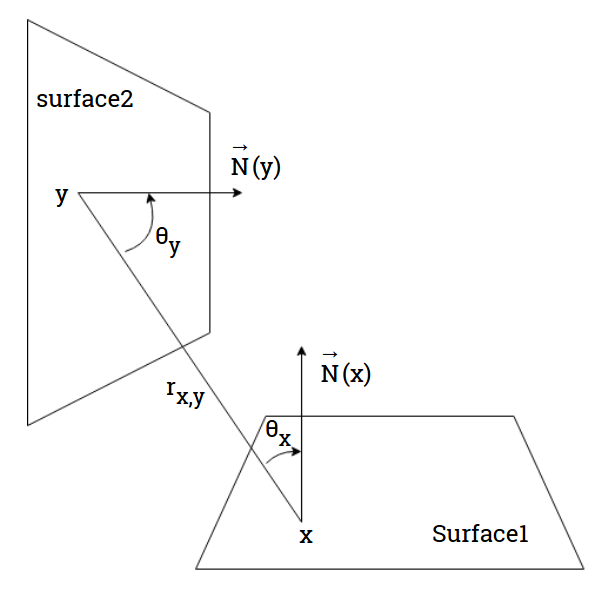
\includegraphics[width=0.4\linewidth]{xy.png}
\caption{This image will be referenced below}
\label{fig:xytheta}
\end{figure}\\
The parameters c and d takes value depending on  the scene. For 2D scenes, a scene consisting of lines instead of surfaces, d takes the value 1 and c takes the value 1/2 and the domain of the points is 1D. In the case of 3D scenes d takes the value 2 and c takes the value 1/$\pi$. From this point onwards we will refer to points by x and depending on the context (1D or  2D) it will be defined. The eq. (\ref{eq:3drie}) can be written as shown in eq. (\ref{eq:genrie})\\\\
{\bf show equation (3)}
\begin{equation} \label{eq:genrie}
B(x)=E(x)+P(x)\int K(x,y)B(y)dy\\\\
\end{equation}
\subsection{Analytical Solution}
In literature lot of methods where developed to solve the non-homogeneous Fredholm integral of second kind[ie survey][other ref]. In particular, if the kernel K is degenerate one can find exact solution of the radiosity integral equation[ie survey]. But for even simple 2D scene the kernel is non degenerate. If analytical solution is not possible then one can solve the problem by approximation methods like Collocation Method, Galerkin Method etc. {\bf But the size of the radiosity problem makes it difficult to use this methods}. We therefor use finite element methods(FEM) to compute approximate solution. We write unknown radiosity function as linear combination of basis function. Thus the problem get casted to system of linear equations which can be solved and approximate solution can be computed.In other words we solve the problem in finite dimensional space(domain). This method is also known as projection methods. More on this is discussed in next section.



\section{Projection methods for radiosity problem}
Radiosity problem was casted to Integral equation but it is very difficult to solve the integral equation analytically due to geometry of scene. We can use projection methods to find approximate solution. We first start with projecting the unknown radiosity function and integrate(operate kernel) on the projected function.\\

{\bf projecting radiosity function}
\subsection{Projecting radiosity function}
Since we are working with linear function spaces and operators
defined on these spaces we must first consider bases. In general
we will be dealing with functions of finite energy, i.e. functions
in the linear vector space $L^2$ . There are many possible bases for
this space. Consider some primal basis $\{N_i \}_{i{\bf belongs to}Z}$ . This set must contain infinitely many functions since $L^2$ is infinite dimensional.
By definition, every function $B{\bf belongs to}L^2$ can be written as a lin-
ear combination of the basis functions $B(x) = \sum _i b_i N_i(x)$ for
some coefficients $b_i$ . In order to find the coefficients of a given
function we need an inner product on $L^2$ . The inner product of
two functions F and G is defined as $<F, G> = \int F(x) G(y) ds$.
Throughout we will denote functions by capital letters. Their expansion coefficients with respect to a basis will be small letters
with indices as subscripts. When denoting functions we will often
drop the argument x (or y).
Given a function B and a set of basis functions $N_i$ , one way
of finding the coefficients of B with respect to this basis is by
performing inner products against the dual basis functions $N{\bf tilde}_i$
dual functions form a basis for the same space, and are defined
through the property\\
$<N_i,N{\bf tilde}_j>=\delta_{ij}$
where $\delta_{ij}$ is the Kronecker Delta. Using the duals we can write
the expansion of a function with respect to a basis as\\

$B(x) = \sum_ib_iN_i(x)= \sum_i<B,N_i>N_i(x)$\\

Now consider a linear operator defined on L 2 . One example is
integration against a kernel function, which is a linear operator since integration is linear. In particular we consider the radiosity
integral equation, which can be written as a linear operator\\

$B=E+KB$\\

where $KB(x) = \int K(x, y)B(y)dy$. Since K is a linear operator it
is fully described by its action on our chosen basis. Intuitively we
can write this as an infinite sized matrix. The columns of the matrix K are given by $KN_j$ . The coefficients of these columns with
respect to our basis can be found by taking inner products with
the dual functions. Thus the entries in the matrix representation
of K are given by\\

$K_{i,j}=<KN_j,N{\bf tilde}_i>=\int \int K(x,y)N_j(y)N{\bf tilde}_i(x)$\\

with this we can write radiosity integral equation as an infinite sized matrix equation\\

$(I-K)B=E$\\

{\bf Show countably finite thing \\ and also show the difference between space and basis for that space}\\

in next section we introduce wavelets and the wavelet basis
\\\\
\section{Wavelets}
Wavelet constitute a family of functions constructed from dilation and translation of a single function called the mother wavelet. When the dilation parameter a and the translation parameter b vary continuously, we have the following family of continuous wavelets as [Boggess]\\

$\psi_{a,b}(x) = {|a|}^{-1} \psi(\frac {t-b}{a})
,   \hspace{0.2cm} a,b \in R, a \neq 0.
$\\

If we restrict the parameters $a$ and $b$ to the discrete values as $a = a_0 ^-k, \\b = n b_0 a_0^{-k}$, where $a>1,b>0$ and $n$, and $k$ are positive integers, we have the following of discrete wavelets:\\

$\psi_n,k(x) = |a|^\frac{k}{2} \psi(a_0^k t - nb_0)$ ,\\
 which from a wavelet basis for $L^2(R)$. In particular, when $a_0 = 2$ and $b_0 = 1$ then $\psi_n,k (x)$ forms an orthonormal basis [Boggess].
 
 {\bf describe all the wavelet i am going to use like haar, llmw, qlmw, CAS 
 plots twoscale elation and vanishing moments and basis set}
 
 
\section{Wavelet radiosity}
I previous sections projection methods and wavelet has been described. Now we describe the use of wavelet basis for projection method and its advantages. 
We first start with the use of our wavelet basis for expanding our unknown radiosity function B(x) as linear combination of wavelet basis.\\

$B(x) = b_{\phi_0}\phi_0(x)+\sum_{i,j}^{\inf,\inf}b_{\psi_{i,j}}\psi_{i,j}(x)$\\,
where $b_{\phi_0}$ and $b_{\psi_{i,j}}$ coefficients are inner products\\
$b_{\psi_{i,j}}=<B(x),psi_{i,j}(x)>$
From inner product point of view, we find that the small coefficients occur because wavelet functions have vanishing moments.
{\bf define vanishing moments}\\

different wavelet have different vanishing moments. For example Haar wavelet have one vanishing moment. Due to this a function which is nearly constant over the support of wavelet basis function will have coefficient value near 0 corresponding to that wavelet basis function. Similarly linear Legendre multi-wavelets have two vanishing moment, hence function nearly linear will have near 0 coefficient corresponding to that wavelet basis function. This is the advantage of using wavelet basis over box function as basis.\\

Once we project the radiosity function into wavelet basis we need to operate the integral on the projected 

Consider a 2D scene consisting of the two line segment of length 1 meter and at distance of 0.5 meter (see figure (2)). \\

{\bf show figue 2}\\

{\bf explain about the kernel sparsity of wavelet projection }\\

{\bf expalin about 2D and 4d wavelet function (tensor product)}
\section{Experiments and results}
In this section comparison of different wavelet with characteristic scenes in 2D(flatland) and 3D has been analyzed. Such a comparison can never be exhaustive due to the heterogeneous nature of input in computer graphics. Therefor scenes with different kind of kernels has been chosen for comparison of performance of our wavelets. We first chose kernels for which we have the exact analytical solution of the integral equation. Then we chose the 2D scenes knows as flatland scenes. For analysis and understanding different aspects of wavelet basis for radiosity we chose 2D scenes. Results of using different wavelet in 3D scenes are also discussed at the end. \\

{\bf Ground truth comparison}\\
For comparing the approximate solution with exact ground truth we chose kernels which are classified as degenerate kernels. Degenerate kernels are kernels which can be expanded in the form shown in eq. (\ref{eq:kxy})
\begin{equation} \label{eq:kxy}
K(x,y) = \sum\limits_{i=1}^na_i(x)b_i(y) \\ 
\end{equation}
An integral equation with degenerate kernel can be solved by changing the order of integral and summation after substituting expanded kernel. See a
appendix A\\

{\bf give proper reference}\\
for analytical solution of non-homogeneous Fredholm IE of second kind. 

We took kernel $K(x,y)=(x-y)^2$ and $K(x,y)=x^4+y^2$ for comparing different wavelets with the ground truth solution $B(x)=${\bf find the solution} of the IE shown in eq. \ref{eq:genrie}

We compare wavelets by calculating error in the projection of kernel $K(x,y)$ and error in solution $B(x)$. The metric used for comparison is relative error as shown in eq. \ref{eq:Krelerr}. It is a ratio of $L^2$ norm of error $(K(x,y)-\hat{K}(x,y))$ to $L^2$ norm of kernel. Where $\hat{K}(x,y)$ is approximation of $K(x,y)$ in space spanned by chosen wavelet.
\begin{equation} \label{eq:Krelerr}
relative  error=\frac{\int\int \,(K(x,y)-\hat{K}(x,y))^2  \,dy \, dx}{\int\int \,K(x,y))^2  \,dy \, dx}
\end{equation}

{\bf flatland}\\

{\bf 4d}\\


\section{conclusion}
\section{Bibliography}
[goral] Modeling the Interaction of Light Between Diffuse Surfaces
Cindy M. Goral, Kenneth E. Torrance, Donald P. Greenberg and Bennett Battaile
Cornell University
Ithaca, New York 14853 \\
\section{appendix}
\subsection{derivation of degenerate kernel}
\end{document}